%%%%%%%%%%%%%%%%%%%%%%%%%%%%%%%%%%%%%%%%%%%%%%%%%%%%%%%%%%%%%%%%%%%%%%%%%%%%%

\begingroup
\renewcommand{\cleardoublepage}{}
\renewcommand{\clearpage}{}
\vspace{1em}
\chapter{Анализ параметров для диагностики дисков}
\endgroup
%%%%%%%%%%%%%%%%%%%%%%%%%%%%%%%%%%%%%%%%%%%%%%%%%%%%%%%%%%%%%%%%%%%%%%%%%%%%%

%%%%%%%%%%%%%%%%%%%%%%%%%%%%%%%%%%%%%%%%%%%%%%%%%%%%%%%%%%%%%%%%%%%%%%%%%%%%%
\section{HDD диски}
%%%%%%%%%%%%%%%%%%%%%%%%%%%%%%%%%%%%%%%%%%%%%%%%%%%%%%%%%%%%%%%%%%%%%%%%%%%%%
Традиционно надежность HDD дисков оценивается на основании метрики MTBF - среднего времени наработки на отказ. Однако, в последнее время, производители перешли к метрике AFR - пересчитанная на год интенсивность отказов. Причина такогого перехода заключается в том, что MTBF рассчитывается с учётом конструкционных особенностей жесткого диска и может быть вычеслена несколькими способами, что приводит к существенно различным результатам. 

Распростаненными оценками MTBF являются 300000-1200000 часов, что соответсвует 30-120 годам беспрерывной работы устройств. Расчет данной метрики производится на основании испытания большого количества дисков, постоянно работающих на испытательной площадке производителя, с последущей экстраполяцией результатов. 

Надежность жесткого диска тесно связана с климатическими параметрами вокруг него. 
Рассмотрим для примера один из используемых HDD дисков - HGST Ultrastar 7K6000~\cite{HGST}. На рисунке ~\ref{fig:temp} приведен график рабочего диапазона температур и высоты над уровнем моря для рассматриваемого диска. Аналогичные показатели с небольшими отклонениями(не более 5 градусов цельсия и 500м высоты) приводят и другие производители, что связано со схожими технологиями производства и применяемыми компонентами. 

\begin{figure}[!h]
	\centering
	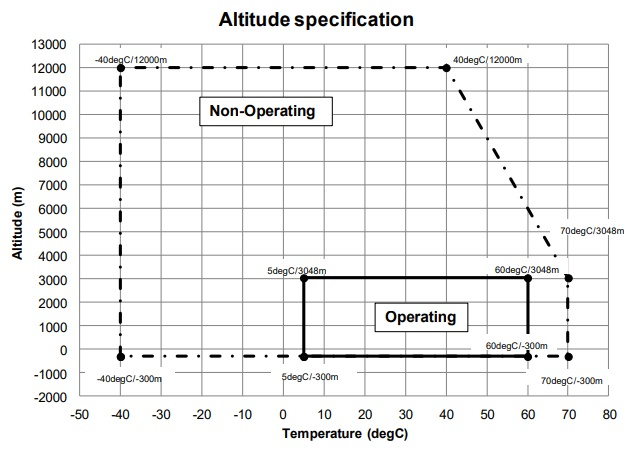
\includegraphics[width=\textwidth]{temp}
	\caption{График предельных значений высоты над уровнем моря от температуры для диска HGST Ultrastar}
	\label{fig:temp}
\end{figure}

Кроме того, важным показателем окружающей среды, влияющим на срок службы жосткого диска является влажность. График рабочих диапазонов влажности от температуры (см. рисунок ~\ref{fig:temp}) демонстрирует резкое снижение рабочего порога влажности при увеличении температуры начиная с 30 градусов цельсия. 

Основываясть на знаниях о принципе действия жестких дисков можно предположить, что такой параметр как уровень вибрации на корпусе диска может также повлиять на срок его службы. Это может быть связано с ускорением износа механической части (подшипников в двигателе, опорных подшипков).

\begin{figure}[!h]
	\centering
	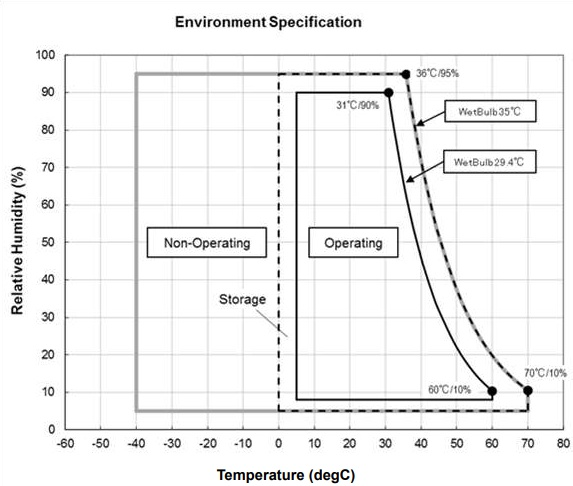
\includegraphics[width=\textwidth]{hum}
	\caption{График предельных значений влажности от температуры для диска HGST Ultrastar}
	\label{fig:hum}
\end{figure}

Таким образом, вышеупомянутые параметры давления(напрямую связано с высотой над уровнем моря), влажности, температуры и вибрации являются важной частью мониторинга состояния HDD дисков. 

Кроме того,... про SMART????
%%%%%%%%%%%%%%%%%%%%%%%%%%%%%%%%%%%%%%%%%%%%%%%%%%%%%%%%%%%%%%%%%%%%%%%%%%%%%
\section{SSD дииски}
%%%%%%%%%%%%%%%%%%%%%%%%%%%%%%%%%%%%%%%%%%%%%%%%%%%%%%%%%%%%%%%%%%%%%%%%%%%%%

В статье ~\cite{reliabil} авторами рассматривается вопрос надёжности SSD дисков, на основании NAND ячейки, произведённых по различным технологиям.

Для ясности дадим определение двум рассматриваемым метрикам:
\begin{itemize*}
	\item{UBER (uncorrectable bit error rate= uncorrectable bit readed/total bit readed}
	\item{RBER (raw bit error rate)= N corrupted bits / N bits readed}
\end{itemize*}
Зачастую, в различных исследованиях и докладах ~\cite{art} о надежности SSD дисков для оценки состояния носителя используется именно эта метрика. 
Однако, метрика UBER не является хорошим инструментом для оценки состояния диска. Алгоритмическое исправление ошибок чаще всего реализовано циклически, поэтому прежде чем ячейка будет исправлена, каждое чтение из неё будет увеличивать значение в числителе. Таким образом числитель и знаменатель коррелируют, вводя в заблуждение исследователей. 

По вышеописанной причине, авторы предлагают использовать метрику RBER. 


Среди результатов исследования также значится:
\begin{itemize*}
	\item{97\% дисков имеет битые ячейки памяти ещё со стадии производства. Их количество зависит от производителя и модели} 
    \item{От 2 до 7\% исследуемых дисков имели бите чипы}
    \item{Чаще всего, в случае одновременного выхода из строя парного количества ячеек, виноват чип} 
    \item{Определены параметры для диагностики состояния диска:}
	\begin{enumerate}
		\item{Ошибки данных (обнаруженные CRC, и пр.)}
		\item{Ошибки чтения/записи}
		\item{Ошибки отключения SATA}
		\item{Количество переназначенных секторов}
	\end{enumerate}
\end{itemize*}

Результаты исследования, с указанием процента устройств, вышедших их строя с обозначенными параметрами, отклоняющимися от нормальных значений, показаны на рисунке ~\ref{fig:failed}. Как видно из рисунка, наиболее точным признаком среди исследованных является количество переназначенных секторов, что напрямую связано с количеством неисправленных бит.
Значение метрики RBER= 1e-08 – 1e-03(чаще всего 1е-06) наблюдалось у устройств, непосредственно перед выходом из строя, а, следовательно, может быть использовано как опорное в целях диагностики состояния диска.

\begin{figure}[h]
	\centering
	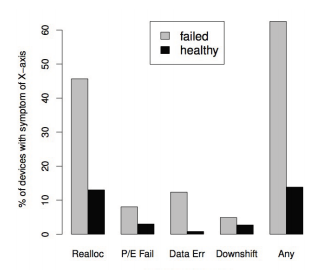
\includegraphics[width=3.0in]{failed}
	\caption{Процент вышедших из строя устройств 
с указанными симптомами}
	\label{fig:failed}
\end{figure}

В статье ~\cite{faildatacenter} исследователи из компании Microsoft также систематизировали возникающие выходы из строя дисков и связали их с наблюдаемыми параметрами. 
В результате, выделяется четыре наиболее важных симптома для определения состояния SSD:
\begin{itemize*}
	\item{Ошибки данных}
    \item{Переназначение секторов}
    \item{Ошибки чтения/записи}
    \item{Ошибки отключения SATA}
\end{itemize*}
Представленный выше набор симптомов сходится с аналогичным набором выше от других исследователей. 
Кроме того, определяется степень важности характеристик для идентификации состояния диска по категориям (см. рисунок ~\ref{fig:params}). 
\begin{figure}[!h]
	\centering
	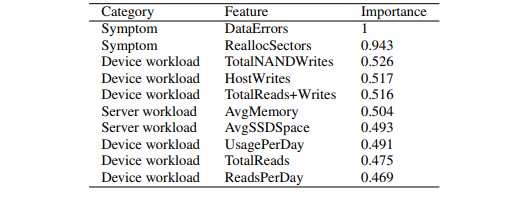
\includegraphics[width=\textwidth]{params}
	\caption{Важность исследуемых характеристик в 
		диагностике состояния устройства}
	\label{fig:params}
\end{figure}

Также в ходе исследования были получены следующие результаты:
\begin{itemize*}
	\item{80\% здоровых устройств имеют <2 переназначенных секторов}
    \item{Если сообщения о сбое основаны на внутренних ошибках/проблемах, то чаще всего устройство выйдет из строя в течении месяца. Если сообщения о сбое основаны на большой нагрузке на устройство – чаще всего устройство функционирует дольше месяца}
    \item{Около 62\% вышедших из строя устройств имеют как минимум один из 4 проявившийся симптом. При этом оставшиеся 38\% не демонстрируют наличие проявления обозначенных симптомов} 
    \item{Определён ряд паттернов на основе различных метрик для оценки состояния диска. Пример представлен на рисунке ~\ref{fig:patterns}. Параметр MediaWearout приведен к шкале 1-100(100- новый диск, 1- полностью изношен)}
\end{itemize*}

\begin{figure}[h]
	\centering
	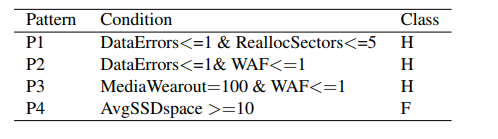
\includegraphics[width=\textwidth]{patterns}
	\caption{Пример паттернов определения состояния диска}
	\label{fig:patterns}
\end{figure}
 

Где WAF - write amplification –отношение количества записанных данных на диск к количеству данных отправленному на запись на хосте.
Графа Class представляет класс, к которому стоит отнести устройство с удовлетворяющими правилу параметрами (H – Healthy-здоровый, F – Failure- неисправный).


Кроме того, в  ~\cite{errorpredr} описано исследование 7 моделей дисков с целью определения параметров, позволяющих определять состояние диска. Кроме упоминаемых ранее, в нем фигурируют такие параметры как ошибки фабрики, недельные статистики циклов записи и количества плохих секторов.
\begin{table}
	\captionsetup{skip=5pt}
	\caption{Агрегированный набор параметров 
		для определения состояния SSD диска}
	\centering
	\begin{tabular}{ | l | l | }
		\hline
		ID & Parameter Name \\ \hline
		1 & correctable error  \\
		2 & erase count \\
		3 & erase error \\
		4 & factory bad blocks\\
		5 & final read error\\
		6 & final write error\\
		7 & meta error\\
		8 & PCI Bus Power Consumotion\\
		9 & read count\\
		10 & read error\\
		11 & response error\\
		12 & status dead\\
		13 & status read only\\
		14 & temperature\\
		15 & timeout error\\
		16 & total NAND writes\\
		17 & uncorrectable error\\
		18 & write count\\
		19 & write error\\
		20 & comulative bad block count fixed\\
		21 & weekly bad block count\\
		22 & comulative program/erase cycle fixed\\
		23 & weekly program/erase cycle\\
		\hline
	\end{tabular}
	\label{table:tab1}
\end{table}

В таблице  ~\ref{table:tab1} представлен агрегированный список параметров составленный на основании рассмотренных статей. Данные параметры представляют наибольший интерес при диагностике SSD дисков. 
